%-----------------------------------------------------------------------------------------
% Autor dieser Vorlage:
% Stefan Macke (http://fachinformatiker-anwendungsentwicklung.net)
% Permalink zur Vorlage: http://fiae.link/LaTeXVorlageFIAE
%
% Sämtliche verwendeten Abbildungen, Tabellen und Listings stammen von Dirk Grashorn.
%
% Lizenz: Creative Commons 4.0 Namensnennung - Weitergabe unter gleichen Bedingungen
% -----------------------------------------------------------------------------------------

\documentclass[
	ngerman,
	toc=listof, % Abbildungsverzeichnis sowie Tabellenverzeichnis in das Inhaltsverzeichnis aufnehmen
	toc=bibliography, % Literaturverzeichnis in das Inhaltsverzeichnis aufnehmen
	footnotes=multiple, % Trennen von direkt aufeinander folgenden Fußnoten
	parskip=half, % vertikalen Abstand zwischen Absätzen verwenden anstatt horizontale Einrückung von Folgeabsätzen
	numbers=noendperiod % Den letzten Punkt nach einer Nummerierung entfernen (nach DIN 5008)
]{scrartcl}

\usepackage[utf8]{inputenc} % muss als erstes eingebunden werden, da Meta/Packages ggfs. Sonderzeichen enthalten

% !TEX root = Projektdokumentation.tex

% Hinweis: der Titel muss zum Inhalt des Projekts passen und den zentralen Inhalt des Projekts deutlich herausstellen
\newcommand{\titel}{Projektplan}
\newcommand{\untertitel}{Heizungssteuerung mit ZigBee}
\newcommand{\kompletterTitel}{\titel{} -- \untertitel}

\newcommand{\autorName}{Eugen Schlecht, Florens Hückstädt, Florian Wohlgemuth, Patrick Wohlgemuth}
\newcommand{\autorAnschrift}{Meine Straße 1}
\newcommand{\autorOrt}{49377 Vechta}

\newcommand{\betriebLogo}{HHN_Logo.png}
\newcommand{\betriebName}{\textsc{Alte Oldenburger} Krankenversicherung AG}
\newcommand{\betriebAnschrift}{Theodor-Heuss-Str. 96}
\newcommand{\betriebOrt}{49377 Vechta}

\newcommand{\ausbildungsberuf}{Software Engineering Bachelor}
\newcommand{\betreff}{Embedded Systems}
\newcommand{\pruefungstermin}{Sommer 2015}
\newcommand{\abgabeOrt}{Vechta}
\newcommand{\abgabeTermin}{23.04.2015}
 % Metadaten zu diesem Dokument (Autor usw.)
% !TEX root = ../Projektdokumentation.tex

% Anpassung an Landessprache ---------------------------------------------------
\usepackage{babel}

% Umlaute ----------------------------------------------------------------------
%   Umlaute/Sonderzeichen wie äüöß direkt im Quelltext verwenden (CodePage).
%   Erlaubt automatische Trennung von Worten mit Umlauten.
% ------------------------------------------------------------------------------
\usepackage[T1]{fontenc}
\usepackage{textcomp} % Euro-Zeichen etc.

% Schrift ----------------------------------------------------------------------
\usepackage{lmodern} % bessere Fonts
\usepackage{relsize} % Schriftgröße relativ festlegen

% Tabellen ---------------------------------------------------------------------
\PassOptionsToPackage{table}{xcolor}
\usepackage{tabularx}
% für lange Tabellen
\usepackage{longtable}
\usepackage{array}
\usepackage{ragged2e}
\usepackage{lscape}
\newcolumntype{w}[1]{>{\raggedleft\hspace{0pt}}p{#1}} % Spaltendefinition rechtsbündig mit definierter Breite

% Grafiken ---------------------------------------------------------------------
\usepackage[dvips,final]{graphicx} % Einbinden von JPG-Grafiken ermöglichen
\usepackage{graphics} % keepaspectratio
\usepackage{floatflt} % zum Umfließen von Bildern
\graphicspath{{Bilder/}} % hier liegen die Bilder des Dokuments

% Sonstiges --------------------------------------------------------------------
\usepackage[titles]{tocloft} % Inhaltsverzeichnis DIN 5008 gerecht einrücken
\usepackage{amsmath,amsfonts} % Befehle aus AMSTeX für mathematische Symbole
\usepackage{enumitem} % anpassbare Enumerates/Itemizes
\usepackage{xspace} % sorgt dafür, dass Leerzeichen hinter parameterlosen Makros nicht als Makroendezeichen interpretiert werden

\usepackage{makeidx} % für Index-Ausgabe mit \printindex
\usepackage[printonlyused]{acronym} % es werden nur benutzte Definitionen aufgelistet

% Einfache Definition der Zeilenabstände und Seitenränder etc.
\usepackage{setspace}
\usepackage{geometry}

% Symbolverzeichnis
\usepackage[intoc]{nomencl}
\let\abbrev\nomenclature
\renewcommand{\nomname}{Abkürzungsverzeichnis}
\setlength{\nomlabelwidth}{.25\hsize}
\renewcommand{\nomlabel}[1]{#1 \dotfill}
\setlength{\nomitemsep}{-\parsep}

\usepackage{varioref} % Elegantere Verweise. „auf der nächsten Seite“
\usepackage{url} % URL verlinken, lange URLs umbrechen etc.

\usepackage{chngcntr} % fortlaufendes Durchnummerieren der Fußnoten
% \usepackage[perpage]{footmisc} % Alternative: Nummerierung der Fußnoten auf jeder Seite neu

\usepackage{ifthen} % bei der Definition eigener Befehle benötigt
\usepackage{todonotes} % definiert u.a. die Befehle \todo und \listoftodos
\usepackage[square]{natbib} % wichtig für korrekte Zitierweise

% PDF-Optionen -----------------------------------------------------------------
\usepackage{pdfpages}
\pdfminorversion=5 % erlaubt das Einfügen von pdf-Dateien bis Version 1.7, ohne eine Fehlermeldung zu werfen (keine Garantie für fehlerfreies Einbetten!)
\usepackage[
    bookmarks,
    bookmarksnumbered,
    bookmarksopen=true,
    bookmarksopenlevel=1,
    colorlinks=true,
% diese Farbdefinitionen zeichnen Links im PDF farblich aus
    linkcolor=AOBlau, % einfache interne Verknüpfungen
    anchorcolor=AOBlau,% Ankertext
    citecolor=AOBlau, % Verweise auf Literaturverzeichniseinträge im Text
    filecolor=AOBlau, % Verknüpfungen, die lokale Dateien öffnen
    menucolor=AOBlau, % Acrobat-Menüpunkte
    urlcolor=AOBlau,
% diese Farbdefinitionen sollten für den Druck verwendet werden (alles schwarz)
    %linkcolor=black, % einfache interne Verknüpfungen
    %anchorcolor=black, % Ankertext
    %citecolor=black, % Verweise auf Literaturverzeichniseinträge im Text
    %filecolor=black, % Verknüpfungen, die lokale Dateien öffnen
    %menucolor=black, % Acrobat-Menüpunkte
    %urlcolor=black,
%
    %backref, % Quellen werden zurück auf ihre Zitate verlinkt
    pdftex,
    plainpages=false, % zur korrekten Erstellung der Bookmarks
    pdfpagelabels=true, % zur korrekten Erstellung der Bookmarks
    hypertexnames=false, % zur korrekten Erstellung der Bookmarks
    linktocpage % Seitenzahlen anstatt Text im Inhaltsverzeichnis verlinken
]{hyperref}
% Befehle, die Umlaute ausgeben, führen zu Fehlern, wenn sie hyperref als Optionen übergeben werden
\hypersetup{
    pdftitle={\titel -- \untertitel},
    pdfauthor={\autorName},
    pdfcreator={\autorName},
    pdfsubject={\titel -- \untertitel},
    pdfkeywords={\titel -- \untertitel},
}


% zum Einbinden von Programmcode -----------------------------------------------
\usepackage{listings}
\usepackage{xcolor}
\definecolor{hellgelb}{rgb}{1,1,0.9}
\definecolor{colKeys}{rgb}{0,0,1}
\definecolor{colIdentifier}{rgb}{0,0,0}
\definecolor{colComments}{rgb}{0,0.5,0}
\definecolor{colString}{rgb}{1,0,0}
\lstset{
    float=hbp,
	basicstyle=\footnotesize,
    identifierstyle=\color{colIdentifier},
    keywordstyle=\color{colKeys},
    stringstyle=\color{colString},
    commentstyle=\color{colComments},
    backgroundcolor=\color{hellgelb},
    columns=flexible,
    tabsize=2,
    frame=single,
    extendedchars=true,
    showspaces=false,
    showstringspaces=false,
    numbers=left,
    numberstyle=\tiny,
    breaklines=true,
    breakautoindent=true,
	captionpos=b,
}
\lstdefinelanguage{cs}{
	sensitive=false,
	morecomment=[l]{//},
	morecomment=[s]{/*}{*/},
	morestring=[b]",
	morekeywords={
		abstract,event,new,struct,as,explicit,null,switch
		base,extern,object,this,bool,false,operator,throw,
		break,finally,out,true,byte,fixed,override,try,
		case,float,params,typeof,catch,for,private,uint,
		char,foreach,protected,ulong,checked,goto,public,unchecked,
		class,if,readonly,unsafe,const,implicit,ref,ushort,
		continue,in,return,using,decimal,int,sbyte,virtual,
		default,interface,sealed,volatile,delegate,internal,short,void,
		do,is,sizeof,while,double,lock,stackalloc,
		else,long,static,enum,namespace,string},
}
\lstdefinelanguage{natural}{
	sensitive=false,
	morecomment=[l]{/*},
	morestring=[b]",
	morestring=[b]',
	alsodigit={-,*},
	morekeywords={
		DEFINE,DATA,LOCAL,END-DEFINE,WRITE,CALLNAT,PARAMETER,USING,
		IF,NOT,END-IF,ON,*ERROR-NR,ERROR,END-ERROR,ESCAPE,ROUTINE,
		PERFORM,SUBROUTINE,END-SUBROUTINE,CONST,END-FOR,END,FOR,RESIZE,
		ARRAY,TO,BY,VALUE,RESET,COMPRESS,INTO,EQ},
}
\lstdefinelanguage{php}{
	sensitive=false,
	morecomment=[l]{/*},
	morestring=[b]",
	morestring=[b]',
	alsodigit={-,*},
	morekeywords={
		abstract,and,array,as,break,case,catch,cfunction,class,clone,const,
		continue,declare,default,do,else,elseif,enddeclare,endfor,endforeach,
		endif,endswitch,endwhile,extends,final,for,foreach,function,global,
		goto,if,implements,interface,instanceof,namespace,new,old_function,or,
		private,protected,public,static,switch,throw,try,use,var,while,xor
		die,echo,empty,exit,eval,include,include_once,isset,list,require,
		require_once,return,print,unset},
}
 % verwendete Packages
% !TEX root = ../Projektdokumentation.tex

% Seitenränder -----------------------------------------------------------------
\setlength{\topskip}{\ht\strutbox} % behebt Warnung von geometry
\geometry{a4paper,left=20mm,right=20mm,top=25mm,bottom=35mm}

\usepackage[
	automark, % Kapitelangaben in Kopfzeile automatisch erstellen
	headsepline, % Trennlinie unter Kopfzeile
	ilines % Trennlinie linksbündig ausrichten
]{scrpage2}

% Kopf- und Fußzeilen ----------------------------------------------------------
\pagestyle{scrheadings}
% chapterpagestyle gibt es nicht in scrartcl
%\renewcommand{\chapterpagestyle}{scrheadings}
\clearscrheadfoot

% Kopfzeile
\renewcommand{\headfont}{\normalfont} % Schriftform der Kopfzeile
\ihead{\large{\textsc{\titel}}\\ \small{\untertitel} \\[2ex] \textit{\headmark}}
\chead{}
\ohead{\includegraphics[scale=0.5]{\betriebLogo}}
\setlength{\headheight}{15mm} % Höhe der Kopfzeile
%\setheadwidth[0pt]{textwithmarginpar} % Kopfzeile über den Text hinaus verbreitern (falls Logo den Text überdeckt)

% Fußzeile
\ifoot{\autorName}
\cfoot{}
\ofoot{\pagemark}

% Überschriften nach DIN 5008 in einer Fluchtlinie
% ------------------------------------------------------------------------------

% Abstand zwischen Nummerierung und Überschrift definieren
% > Schön wäre hier die dynamische Berechnung des Abstandes in Abhängigkeit
% > der Verschachtelungstiefe des Inhaltsverzeichnisses
\newcommand{\headingSpace}{1.5cm}

% Abschnittsüberschriften im selben Stil wie beim Inhaltsverzeichnis einrücken
\renewcommand*{\othersectionlevelsformat}[3]{
  \makebox[\headingSpace][l]{#3\autodot}
}

% Für die Einrückung wird das Paket tocloft benötigt
%\cftsetindents{chapter}{0.0cm}{\headingSpace}
\cftsetindents{section}{0.0cm}{\headingSpace}
\cftsetindents{subsection}{0.0cm}{\headingSpace}
\cftsetindents{subsubsection}{0.0cm}{\headingSpace}
\cftsetindents{figure}{0.0cm}{\headingSpace}
\cftsetindents{table}{0.0cm}{\headingSpace}


% Allgemeines
% ------------------------------------------------------------------------------

\onehalfspacing % Zeilenabstand 1,5 Zeilen
\frenchspacing % erzeugt ein wenig mehr Platz hinter einem Punkt

% Schusterjungen und Hurenkinder vermeiden
\clubpenalty = 10000
\widowpenalty = 10000
\displaywidowpenalty = 10000

% Quellcode-Ausgabe formatieren
\lstset{numbers=left, numberstyle=\tiny, numbersep=5pt, breaklines=true}
\lstset{emph={square}, emphstyle=\color{red}, emph={[2]root,base}, emphstyle={[2]\color{blue}}}

\counterwithout{footnote}{section} % Fußnoten fortlaufend durchnummerieren
\setcounter{tocdepth}{\subsubsectionlevel} % im Inhaltsverzeichnis werden die Kapitel bis zum Level der subsubsection übernommen
\setcounter{secnumdepth}{\subsubsectionlevel} % Kapitel bis zum Level der subsubsection werden nummeriert

% Aufzählungen anpassen
\renewcommand{\labelenumi}{\arabic{enumi}.}
\renewcommand{\labelenumii}{\arabic{enumi}.\arabic{enumii}.}
\renewcommand{\labelenumiii}{\arabic{enumi}.\arabic{enumii}.\arabic{enumiii}}

% Tabellenfärbung:
\definecolor{heading}{rgb}{0.64,0.78,0.86}
\definecolor{odd}{rgb}{0.9,0.9,0.9}
 % Definitionen zum Aussehen der Seiten
% !TEX root = ../Projektdokumentation.tex

% Abkürzungen, ggfs. mit korrektem Leerraum
\newcommand{\bs}{$\backslash$\xspace}
\newcommand{\bspw}{bspw.\xspace}
\newcommand{\bzw}{bzw.\xspace}
\newcommand{\ca}{ca.\xspace}
\newcommand{\dahe}{\mbox{d.\,h.}\xspace}
\newcommand{\etc}{etc.\xspace}
\newcommand{\eur}[1]{\mbox{#1\,\texteuro}\xspace}
\newcommand{\evtl}{evtl.\xspace}
\newcommand{\ggfs}{ggfs.\xspace}
\newcommand{\Ggfs}{Ggfs.\xspace}
\newcommand{\gqq}[1]{\glqq{}#1\grqq{}}
\newcommand{\inkl}{inkl.\xspace}
\newcommand{\insb}{insb.\xspace}
\newcommand{\ua}{\mbox{u.\,a.}\xspace}
\newcommand{\usw}{usw.\xspace}
\newcommand{\Vgl}{Vgl.\xspace}
\newcommand{\zB}{\mbox{z.\,B.}\xspace}

% Befehle für häufig anfallende Aufgaben
\newcommand{\Abbildung}[1]{\autoref{fig:#1}}
\newcommand{\Anhang}[1]{\appendixname{}~\ref{#1}: \nameref{#1} \vpageref{#1}}
\newcommand{\includegraphicsKeepAspectRatio}[2]{\includegraphics[width=#2\textwidth,height=#2\textheight,keepaspectratio]{#1}}
\newcommand{\Zitat}[2][\empty]{\ifthenelse{\equal{#1}{\empty}}{\citep{#2}}{\citep[#1]{#2}}}
\newcommand{\Autor}[1]{\textsc{#1}} % zum Ausgeben von Autoren
\newcommand{\itemd}[2]{\item{\textbf{#1}}\\{#2}} % erzeugt ein Listenelement mit fetter Überschrift

% fügt Tabellen aus einer TEX-Datei ein
\newcommand{\tabelle}[3] % Parameter: caption, label, file
{\begin{table}[htbp]
\centering
\singlespacing
\input{Tabellen/#3}
\caption{#1}
\label{#2}
\end{table}}

\newcommand{\tabelleAnhang}[1] % Parameter: file
{\begin{center}
\singlespacing
\input{Tabellen/#1}
\end{center}}

% einfaches Wechseln der Schrift, z.B.: \changefont{cmss}{sbc}{n}
\newcommand{\changefont}[3]{\fontfamily{#1} \fontseries{#2} \fontshape{#3} \selectfont}

% Verwendung analog zu \includegraphics
\newlength{\myx} % Variable zum Speichern der Bildbreite
\newlength{\myy} % Variable zum Speichern der Bildhöhe
\newcommand\includegraphicstotab[2][\relax]{%
% Abspeichern der Bildabmessungen
\settowidth{\myx}{\includegraphics[{#1}]{#2}}%
\settoheight{\myy}{\includegraphics[{#1}]{#2}}%
% das eigentliche Einfügen
\parbox[c][1.1\myy][c]{\myx}{%
\includegraphics[{#1}]{#2}}%
}

\definecolor{AOBlau}{rgb}{0, 0.28, 0.56}

% verschiedene Befehle um Wörter semantisch auszuzeichnen ----------------------
\newcommand{\Index}[2][\empty]{\ifthenelse{\equal{#1}{\empty}}{\index{#2}#2}{\index{#1}#2}}
\newcommand{\Fachbegriff}[2][\empty]{\ifthenelse{\equal{#1}{\empty}}{\textit{\Index{#2}}}{\textit{\Index[#1]{#2}}}}
\newcommand{\NeuerBegriff}[2][\empty]{\ifthenelse{\equal{#1}{\empty}}{\textbf{\Index{#2}}}{\textbf{\Index[#1]{#2}}}}

\newcommand{\Ausgabe}[1]{\texttt{#1}}
\newcommand{\Eingabe}[1]{\texttt{#1}}
\newcommand{\Code}[1]{\texttt{#1}}
\newcommand{\Datei}[1]{\texttt{#1}}

\newcommand{\Assembly}[1]{\textsf{#1}}
\newcommand{\Klasse}[1]{\textsf{#1}}
\newcommand{\Methode}[1]{\textsf{#1}}
\newcommand{\Attribut}[1]{\textsf{#1}}

\newcommand{\Datentyp}[1]{\textsf{#1}}
\newcommand{\XMLElement}[1]{\textsf{#1}}
\newcommand{\Webservice}[1]{\textsf{#1}}

\newcommand{\Refactoring}[1]{\Fachbegriff{#1}}
\newcommand{\CodeSmell}[1]{\Fachbegriff{#1}}
\newcommand{\Metrik}[1]{\Fachbegriff{#1}}
\newcommand{\DesignPattern}[1]{\Fachbegriff{#1}}
 % eigene allgemeine Befehle, die z.B. die Arbeit mit LaTeX erleichtern
% !TEX root = ../Projektdokumentation.tex

% Abkürzungen, ggfs. mit korrektem Leerraum
\newcommand{\bs}{$\backslash$\xspace}
\newcommand{\bspw}{bspw.\xspace}
\newcommand{\bzw}{bzw.\xspace}
\newcommand{\ca}{ca.\xspace}
\newcommand{\dahe}{\mbox{d.\,h.}\xspace}
\newcommand{\etc}{etc.\xspace}
\newcommand{\eur}[1]{\mbox{#1\,\texteuro}\xspace}
\newcommand{\evtl}{evtl.\xspace}
\newcommand{\ggfs}{ggfs.\xspace}
\newcommand{\Ggfs}{Ggfs.\xspace}
\newcommand{\gqq}[1]{\glqq{}#1\grqq{}}
\newcommand{\inkl}{inkl.\xspace}
\newcommand{\insb}{insb.\xspace}
\newcommand{\ua}{\mbox{u.\,a.}\xspace}
\newcommand{\usw}{usw.\xspace}
\newcommand{\Vgl}{Vgl.\xspace}
\newcommand{\zB}{\mbox{z.\,B.}\xspace}

% Befehle für häufig anfallende Aufgaben
\newcommand{\Abbildung}[1]{\autoref{fig:#1}}
\newcommand{\Anhang}[1]{\appendixname{}~\ref{#1}: \nameref{#1} \vpageref{#1}}
\newcommand{\includegraphicsKeepAspectRatio}[2]{\includegraphics[width=#2\textwidth,height=#2\textheight,keepaspectratio]{#1}}
\newcommand{\Zitat}[2][\empty]{\ifthenelse{\equal{#1}{\empty}}{\citep{#2}}{\citep[#1]{#2}}}
\newcommand{\Autor}[1]{\textsc{#1}} % zum Ausgeben von Autoren
\newcommand{\itemd}[2]{\item{\textbf{#1}}\\{#2}} % erzeugt ein Listenelement mit fetter Überschrift

% fügt Tabellen aus einer TEX-Datei ein
\newcommand{\tabelle}[3] % Parameter: caption, label, file
{\begin{table}[htbp]
\centering
\singlespacing
\input{Tabellen/#3}
\caption{#1}
\label{#2}
\end{table}}

\newcommand{\tabelleAnhang}[1] % Parameter: file
{\begin{center}
\singlespacing
\input{Tabellen/#1}
\end{center}}

% einfaches Wechseln der Schrift, z.B.: \changefont{cmss}{sbc}{n}
\newcommand{\changefont}[3]{\fontfamily{#1} \fontseries{#2} \fontshape{#3} \selectfont}

% Verwendung analog zu \includegraphics
\newlength{\myx} % Variable zum Speichern der Bildbreite
\newlength{\myy} % Variable zum Speichern der Bildhöhe
\newcommand\includegraphicstotab[2][\relax]{%
% Abspeichern der Bildabmessungen
\settowidth{\myx}{\includegraphics[{#1}]{#2}}%
\settoheight{\myy}{\includegraphics[{#1}]{#2}}%
% das eigentliche Einfügen
\parbox[c][1.1\myy][c]{\myx}{%
\includegraphics[{#1}]{#2}}%
}

\definecolor{AOBlau}{rgb}{0, 0.28, 0.56}

% verschiedene Befehle um Wörter semantisch auszuzeichnen ----------------------
\newcommand{\Index}[2][\empty]{\ifthenelse{\equal{#1}{\empty}}{\index{#2}#2}{\index{#1}#2}}
\newcommand{\Fachbegriff}[2][\empty]{\ifthenelse{\equal{#1}{\empty}}{\textit{\Index{#2}}}{\textit{\Index[#1]{#2}}}}
\newcommand{\NeuerBegriff}[2][\empty]{\ifthenelse{\equal{#1}{\empty}}{\textbf{\Index{#2}}}{\textbf{\Index[#1]{#2}}}}

\newcommand{\Ausgabe}[1]{\texttt{#1}}
\newcommand{\Eingabe}[1]{\texttt{#1}}
\newcommand{\Code}[1]{\texttt{#1}}
\newcommand{\Datei}[1]{\texttt{#1}}

\newcommand{\Assembly}[1]{\textsf{#1}}
\newcommand{\Klasse}[1]{\textsf{#1}}
\newcommand{\Methode}[1]{\textsf{#1}}
\newcommand{\Attribut}[1]{\textsf{#1}}

\newcommand{\Datentyp}[1]{\textsf{#1}}
\newcommand{\XMLElement}[1]{\textsf{#1}}
\newcommand{\Webservice}[1]{\textsf{#1}}

\newcommand{\Refactoring}[1]{\Fachbegriff{#1}}
\newcommand{\CodeSmell}[1]{\Fachbegriff{#1}}
\newcommand{\Metrik}[1]{\Fachbegriff{#1}}
\newcommand{\DesignPattern}[1]{\Fachbegriff{#1}}
 % eigene projektspezifische Befehle, z.B. Abkürzungen usw.

\begin{document}


\phantomsection
\thispagestyle{plain}
\pdfbookmark[1]{Deckblatt}{deckblatt}
% !TEX root = Projektdokumentation.tex
\begin{titlepage}

\begin{center}

\includegraphics[scale=1.2]{HHN_Logo.png}\\[4ex]


\Large{\ausbildungsberuf}\\
\LARGE{\betreff}\\[4ex]

\huge{\textbf{\titel}}\\[1.5ex]
\Large{\textbf{\untertitel}}\\[4ex]

\normalsize


\autorName\\


\end{center}


\end{titlepage}
\cleardoublepage

% Preface --------------------------------------------------------------------
\phantomsection
\pagenumbering{Roman}
\pdfbookmark[1]{Inhaltsverzeichnis}{inhalt}
\tableofcontents
\cleardoublepage

\phantomsection
\listoffigures
\cleardoublepage

%\phantomsection
%\listoftables
%\cleardoublepage

%\phantomsection
%\lstlistoflistings
%\cleardoublepage



\newcommand{\abkvz}{Abkürzungsverzeichnis}
\renewcommand{\nomname}{\abkvz}
\section*{\abkvz}
\markboth{\abkvz}{\abkvz}
\addcontentsline{toc}{section}{\abkvz}
% !TEX root = Projektdokumentation.tex

% Es werden nur die Abkürzungen aufgelistet, die mit \ac definiert und auch benutzt wurden. 
%
% \acro{VERSIS}{Versicherungsinformationssystem\acroextra{ (Bestandsführungssystem)}}
% Ergibt in der Liste: VERSIS Versicherungsinformationssystem (Bestandsführungssystem)
% Im Text aber: \ac{VERSIS} -> Versicherungsinformationssystem (VERSIS)

% Hinweis: allgemein bekannte Abkürzungen wie z.B. bzw. u.a. müssen nicht ins Abkürzungsverzeichnis aufgenommen werden
% Hinweis: allgemein bekannte IT-Begriffe wie Datenbank oder Programmiersprache müssen nicht erläutert werden,
%          aber ggfs. Fachbegriffe aus der Domäne des Prüflings (z.B. Versicherung)

% Die Option (in den eckigen Klammern) enthält das längste Label oder
% einen Platzhalter der die Breite der linken Spalte bestimmt.
\begin{acronym}[WWWWW]
	\acro{AO}{\textsc{Alte Oldenburger} Krankenversicherung AG}
	\acro{API}{Application Programming Interface}
	\acro{CSS}{Cascading Style Sheets}
	\acro{CSV}{Comma Separated Value}
	\acro{EPK}{Ereignisgesteuerte Prozesskette}
	\acro{ERM}{En\-ti\-ty-Re\-la\-tion\-ship-Mo\-dell}
	\acro{HTML}{Hypertext Markup Language}\acused{HTML}
	\acro{IDE}{Integrated Development Environment}
	\acro{MVC}[MVC]{Model View Controller}
	\acro{NatInfo}[\textsc{NatInfo}]{Natural Information System}
	\acro{Natural}[\textsc{Natural}]{Programmiersprache der Software AG}\acused{Natural}
	\acro{ORM}{Object-Relational Mapping}
	\acro{PHP}{Hypertext Preprocessor}
	\acro{SDK}{Software Development Kit}
	\acro{SQL}{Structured Query Language}
	\acro{SVN}{Subversion}
	\acro{UML}{Unified Modeling Language}
	\acro{XML}{Extensible Markup Language}
	\acro{AT Mode}{Transparent Mode}
	\acro{API Mode}{Application Programming Interface Mode}
	\acro{Rx-Schnittstell}{Receiver-Schnittstelle}
	\acro{Tx-Schnittstell}{Transmitter-Schnittstelle}
\end{acronym}

\clearpage

% Inhalt ---------------------------------------------------------------------
\pagenumbering{arabic}
% !TEX root = Projektdokumentation.tex
\section{Einführung}
Im Zuge der Vorlesung \betreff\ des Studiengangs \ausbildungsberuf\ wird ein Projekt im Bereich der Heimautomatisierung durchgeführt.
Thema des Projekts ist die Konzeption und Erstellung einer Heizungssteuerung. Dabei wird an einem im Sommersemester 2015 durchgeführten Projekt angeknüpft.

\section{Ausgangssituation}

\section{Zieldefinition}\label{Zieldefinition}
Gegenstand des Projekts ist die Weiterführung des über mehrere Semester bearbeitete Thema Hausautomatisierung mit ZigBee. Der Stand der Vorgruppe ist ein durchgeführter Proof-Of-Concept mit Entwicklung eines prototypischen Systems zur Steuerung eines Heizungsventils. Die Absicht der Weiterführung des Themas ist Verarbeitung der gewonnen Erkenntnisse und die Entwicklung eines einsetzbaren Hausautomatisierungssystems. Der Aspekt der Einsetzbarkeit ist dabei so definiert, dass das System Gütekriterien aktueller Produkte im Bereich der Hausautomatisierung entspricht. Als exemplarisches Endgerät, das über das System angesteuert werden kann, bleibt weiterhin das Heizungsventil im Fokus. Der Anspruch an dieses ist nun die Kapselung der Elektronik in ein geschlossenes Gehäuse, so dass ein Anschluss an einen Heizkörper möglich ist. Ein Überblick des Systems inform eines Use-Case-Diagramms ist in \Abbildung{UC} dargestellt. Im Folgendem werden die Teilziele bzw. die Gütekriterien des geplanten Systems erläutert.
\subsection{Erweiterbarkeit}\label{Ziel_Erw}
Die Erweiterbarkeit des Systems beinhaltet zum einen die Möglichkeit der Ansteuerung vielfältiger Endgeräte wie zum Beispiel Lichtschalter, Türöffner, Jalousien. Die Erweiterbarkeit in diesem Sinne erfordert generische Ansätze in den Bereichen der Kommunikation, Datenhaltung und Darstellung. Zum anderen wird Erweiterbarkeit verstanden als Möglichkeit das Softwaresystem ohne großen Aufwand um neue Anforderungen, wie zum Beispiel die Entwicklung von Benutzeroberflächen für verschiedene Endgeräte, zu ergänzen.
\subsection{Benutzerfreundlichkeit}\label{Ziel_Ben}
Die Bedienung, Installation und Erweiterung des Systems soll für den Benutzer möglichst einfach erlernbar sein. Die Benutzeroberflächen sollen dabei an Benutzer angepasst werden, die über keine internen Systemkenntnisse verfügen.
\subsection{Sicherheit}\label{Ziel_Sic}
Das System soll gegen unbefugten Zugriff von außen abgesichert sein. Komponenten der Hausautomatisierung dürfen nicht von Unberechtigten gesteuert werden können.

\begin{figure}[htb]
\centering
\includegraphicsKeepAspectRatio{useCase.png}{0.9}
\caption{Use-Case-Diagramm Heizungssteuerung}
\label{fig:UC}
\end{figure}

\section{Architektur und Umsetzung}

Im Nachfolgenden werden die entwickelten und eingesetzten Lösungen zu den im \autoref{Zieldefinition} beschriebenen hardware- und softwarespezifischen Anforderungen erläutert. \Abbildung{DD} zeigt
die grobe Systemarchitektur der entwickelten Lösung.


\begin{figure}[htb]
\centering
\includegraphicsKeepAspectRatio{deploymentDiagram.png}{0.9}
\caption{Sestemarchitektur}
\label{fig:DD}
\end{figure}

Das System besteht im wesentlichen aus vier Komponenten:

\begin{itemize}
\item \textbf{Endgerät:} Zum Beispiel Heizung, Schalter, Türöffner
\item \textbf{Raumserver:} Steuert Endgerät über das ZigBee-Protokoll
\item \textbf{Cloud Backend:} Bietet eine RESTful API zur Verwaltung der Räume und Geräte
\item \textbf{Web Frontend:} Grafische Oberfläche zur Kommunikation mit dem Cloud Backend
\end{itemize}

Die einzelnen Bestandteile des Systems werden in den folgenden Unterkapiteln genau beschrieben. 

\subsubsection{Backend}
Das Backend kann über ein API von der App angesprochen werden, um Räume und Geräte zu verwalten und Kommandos an diese zu versenden.

\paragraph{API}\mbox{}\\
Das API ist als RESTful Web Service realisiert. Ressourcen können über HTTP mit den Methoden \colorbox{pregray}{\lstinline{GET}}, \colorbox{pregray}{\lstinline{POST}}, \colorbox{pregray}{\lstinline{PUT}} und \colorbox{pregray}{\lstinline{DELETE}} angesprochen werden. Eine genaue Auflistung der API-Methoden ist im Anhang zu finden.

\paragraph{Schema}\mbox{}\\
Sämtlicher Zugriff auf das API erfolgt über HTTPS und kann über \colorbox{pregray}{\lstinline{https://enigmatic-waters-31128.herokuapp.com}} erreicht werden.

\vspace{2em}
\begin{lstlisting}
$ curl 'https://enigmatic-waters-31128.herokuapp.com/api/rooms/d934eb20-4c6f-4d1c-91c5-61cdeddcf843' 
-i -H 'X-AUTH-TOKEN: TOKEN'

HTTP/1.1 200 OK
Connection: keep-alive
Server: Apache-Coyote/1.1
Access-Control-Allow-Origin: *
Access-Control-Allow-Methods: POST, PUT, PATCH, GET, OPTIONS, DELETE
Access-Control-Max-Age: 3600
Access-Control-Allow-Headers: x-requested-with, content-type, X-AUTH-TOKEN
Access-Control-Expose-Headers: X-AUTH-TOKEN
X-Content-Type-Options: nosniff
X-Xss-Protection: 1; mode=block
Cache-Control: no-cache, no-store, max-age=0, must-revalidate
Pragma: no-cache
Expires: 0
Strict-Transport-Security: max-age=31536000 ; includeSubDomains
X-Frame-Options: DENY
Content-Type: application/json;charset=UTF-8
Transfer-Encoding: chunked
Date: Sun, 01 May 2016 10:57:10 GMT
Via: 1.1 vegur

{
  "roomId":"d934eb20-4c6f-4d1c-91c5-61cdeddcf843",
  "name":"Wohnzimmer"
}
\end{lstlisting}
\vspace{2em}

Sowohl beim Abfragen einer Liste als auch beim Abfragen einzelner Ressourcen beinhaltet die Antwort alle Attribute der Ressource.

\subparagraph{Authentifizierung}\mbox{}\\
Anfragen, die eine Authentifizierung erfordern, geben als Antwort \colorbox{pregray}{\lstinline{403 Forbidden}} zurück. Zur Authentifizierung muss im Header das Feld \colorbox{pregray}{\lstinline{X-AUTH-TOKEN}} gesetzt sein. Das entsprechende Token wird nach einer erfolgreichen Login-Anfrage erhalten.

\paragraph{Authentifizierung mit einem Token}\mbox{}\\
\begin{lstlisting}
$ curl 'https://enigmatic-waters-31128.herokuapp.com' -i -H 'X-AUTH-TOKEN: TOKEN'
\end{lstlisting}

\subparagraph{Login}\mbox{}\\
Zum Erhalt eines Tokens muss eine Loginanfrage gestellt werden. Diese enthält die Attribute username und password.
\vspace{2em}
\begin{lstlisting}
$ curl 'https://enigmatic-waters-31128.herokuapp.com/api/login' -i -X POST -H 'Content-Type: application/json' -d '{"username":"foo", "password": "bar"}'

HTTP/1.1 200 OK
Connection: keep-alive
Server: Apache-Coyote/1.1
Access-Control-Allow-Origin: *
Access-Control-Allow-Methods: POST, PUT, PATCH, GET, OPTIONS, DELETE
Access-Control-Max-Age: 3600
Access-Control-Allow-Headers: x-requested-with, content-type, X-AUTH-TOKEN
Access-Control-Expose-Headers: X-AUTH-TOKEN
X-Content-Type-Options: nosniff
X-Xss-Protection: 1; mode=block
Cache-Control: no-cache, no-store, max-age=0, must-revalidate
Pragma: no-cache
Expires: 0
Strict-Transport-Security: max-age=31536000 ; includeSubDomains
X-Frame-Options: DENY
X-Auth-Token: eyJpZCI6MTEsInVzZXJuYW1lIjoidXNlciIsImV4cGlyZXMiOjE0NjI5Njk0NzIwMTgsInJvbGVzIjpbIlVTRVIiXX0=.LDd74G0yJAuQChYR9P0AOmThfylOGGlY19u2DcTcXyQ=
Content-Length: 0
Date: Sun, 01 May 2016 12:24:32 GMT
Via: 1.1 vegur
\end{lstlisting}
\vspace{2em}
Das Token aus dem Response-Header-Feld \colorbox{pregray}{\lstinline{X-AUTH-TOKEN}} muss bei zukünftigen Anfragen enthalten sein.

\paragraph{Fehlgeschlagener Login}\mbox{}\\
Loginanfragen mit ungültigen Benutzerdaten werden mit \colorbox{pregray}{\lstinline{401 Unauthorized}} beantwortet.
\vspace{2em}
\begin{lstlisting}
$ curl 'https://enigmatic-waters-31128.herokuapp.com/api/login' -i -X POST -H 'Content-Type: application/json' -d '{"username":"foo", "password": "bar"}'

HTTP/1.1 401 Unauthorized
Connection: keep-alive
Server: Apache-Coyote/1.1
Access-Control-Allow-Origin: *
Access-Control-Allow-Methods: POST, PUT, PATCH, GET, OPTIONS, DELETE
Access-Control-Max-Age: 3600
Access-Control-Allow-Headers: x-requested-with, content-type, X-AUTH-TOKEN
Access-Control-Expose-Headers: X-AUTH-TOKEN
X-Content-Type-Options: nosniff
X-Xss-Protection: 1; mode=block
Cache-Control: no-cache, no-store, max-age=0, must-revalidate
Pragma: no-cache
Expires: 0
Strict-Transport-Security: max-age=31536000 ; includeSubDomains
X-Frame-Options: DENY
Content-Type: application/json;charset=UTF-8
Transfer-Encoding: chunked
Date: Sun, 01 May 2016 12:30:03 GMT
Via: 1.1 vegur

{
  "timestamp":1462105803298,
  "status":401,
  "error":"Unauthorized",
  "message":"Authentication Failed: Bad credentials",
  "path":"/api/login"
}
\end{lstlisting}


\subsection{Raumserver}\label{Raumserver}
Der Raumserver ist eine Java-Anwendung zur Steuerung von Geräten über ZigBee. Seine Befehle nimmt er über eine Message-Queue entgegen (siehe \autoref{Messaging}. Diese kann vom Benutzer über die Hausautomatisierungs-API vom Cloud Backend angesprochen werden. Der Raumserver bietet darüberhinaus eine Webseite zur Konfiguration (siehe \autoref{RoomConfig}). Zur Kommunikation mit ZigBee-fähigen Geräten wird ein generisches Protokoll verwendet (\autoref{Protokoll}). Der Raspberry Pi dient als Plattform für die Software. Am Raspberry Pi ist ein Temperatursensor verbaut, der vom Raumserver verwendet wird um die Raumtemperatur zu regulieren.

\subsubsection{Hardware}\label{Raum_Hardware}
In folgendem Abschnitt wird auf die hardwarespezifischen Besonderheiten des Raumservers eingegangen. Dabei wird in \autoref{Pi} auf die Plattform eingegangen auf der die Java-Anwendung ausgeführt wird. \autoref{Temp} beschreibt den Temperatursensor, der auf dem Pi verbaut ist. In \autoref{Raum_XBee} wird auf die Hardware eingegangen, die verwendet wird um über das ZigBee-Protokoll mit den Endgeräten zu kommunizieren. Abschließend wird in \autoref{Raum_LED} die Bedeutung der LED-Anzeigen erleutert.
\paragraph{Raspberry Pi}\mbox{}\\\label{Pi}

\paragraph{Temperatursensor}\mbox{}\\\label{Temp}

\paragraph{XBee USB Module}\mbox{}\\\label{Raum_XBee}

\paragraph{Status-LED}\mbox{}\\\label{Raum_LED}


\subsubsection{Software}\label{Raum_Software}

\subsubsection{Schnittstellen}\label{Raum_Schnittstellen}
Der Raumserver bietet mehrere Schnittstellen. Eine Übersicht ist in \Abbildung{RSSS} dargestellt. Dabei wird ein Heizungsventil beipielhaft als Endgerät angegeben.
Der Raumserver kommuniziert mit dem Cloud Backend über die bereitgestellte REST API (siehe \autoref{API}) mittels HTTPS. Über diesen Kanal werden vorwiegend Registrierungen von Endgeräten und Werteänderungen übertragen. Damit der Raumserver mit dem Cloud Backend kommunizieren kann muss er sich bei diesem authentifizieren. Dazu muss der jeweilige Cloud Account des Benutzers über die Konfigurationsseite des Raumservers eingetragen werden (siehe \autoref{RoomConfig}).

Die entgegengesetzte Kommunikation findet über das Messaging-Verfahren AMQP\footnote{https://www.amqp.org/} statt. Die Adressierung der Message Queues geschieht über die eindeutige ID der Raumserver. Die Queues sind persistent. Das heißt für den Fall, dass der Raumserver nicht erreichbar ist, bleiben die Nachrichten bestehen. Der Nachrichteninhalt ist im JSON-Fromat. Siehe dazu folgendes Beispiel:
\vspace{2em}
\begin{lstlisting}
{
   "deviceId": "123",
   "targetValue: "20.5"
}

\end{lstlisting}
\vspace{2em}
Nachrichten beschränken sich auf das Setzen von Werten für bestimmte Endgeräte. Das jeweilige Endgerät wird über die im JSON mitgelieferte deviceId identifiziert. Beim Raumserver eingehende Nachrichten werden an die entsprechenden Endgeräte über das ZigBee-Protokoll weitergeleitet (siehe dazu \autoref{ZigBee}). 

\begin{figure}[htb]
\centering
\includegraphicsKeepAspectRatio{Raumserver_Com.png}{0.6}
\caption{Schnittstellen des Raumservers}
\label{fig:RSSS}
\end{figure}

Innerhalb der ZigBee-Kommunikation nimmt der Raumserver die Rolle des Coordinator\footnote{https://en.wikipedia.org/wiki/ZigBee} ein und die Geräte wie zum Beispiel das Heizungsventil die Rolle des End Device (siehe \Abbildung{CBRSED}).

\begin{figure}[htb]
\centering
\includegraphicsKeepAspectRatio{rooms_graph2.png}{0.6}
\caption{ZigBee-Netzwerk mit Raumserver und Geräten}
\label{fig:CBRSED}
\end{figure}

\subsubsection{Konfiguration}\label{RoomConfig}

\begin{figure}[htb]
\centering
\includegraphicsKeepAspectRatio{Config.png}{1.0}
\caption{Konfigurationsseite des Raumservers}
\label{fig:ConfigRaum}
\end{figure}

\begin{figure}[htb]
\centering
\includegraphicsKeepAspectRatio{ConfigLogin.png}{1.0}
\caption{Eingabemaske für den Cloud Account}
\label{fig:ConfigRaum_Login}
\end{figure}






\subsubsection{Nachrichtenprotokoll}\label{Protokoll}

\begin{figure}[htb]
\centering
\includegraphicsKeepAspectRatio{protokoll.png}{0.6}
\caption{Raumserver XBee-Nachrichtenstruktur}
\label{fig:Frame}
\end{figure}


\begin{table}[]
\centering
\begin{tabular}{|l|l|l|l|}
\hline
\textbf{CMD} & \textbf{Bezeichnung} & \textbf{ARG1} & \textbf{ARG2} \\ \hline
01            & Wert setzen          & Wert          &               \\ \hline
02            & Statusanfrage        &               &               \\ \hline
03            & Status               & Gerätetype    & Wert          \\ \hline
\end{tabular}
\caption{Komanndotypen}
\label{CMDS}
\end{table}
\begin{table}[]
\centering
\begin{tabular}{|l|l|}
\hline
\textbf{Gerätetypen} & \textbf{Bezeichnung} \\ \hline
01                    & Heizung           \\ \hline
02                    & Schalter             \\ \hline
\end{tabular}
\caption{Gerätetypen}
\label{Devices}
\end{table}

\begin{table}[]
\centering
\begin{tabular}{|l|l|l|}
\hline
\textbf{CMD}                  & \textbf{ARG1}                 & \textbf{ARG2}                \\ \hline
\multicolumn{3}{|l|}{Statusanfrage}                                                          \\ \hline
02                            & 00                            & 00                           \\ \hline
\multicolumn{3}{|l|}{Statusantwort: Gerät ist Heizung mit Wert 0 =\textgreater geschlossen}  \\ \hline
03                            & 01                            & 00                           \\ \hline
\multicolumn{3}{|l|}{Heizung 5\% öffnen}                                                     \\ \hline
01                            & 05                            & 00                           \\ \hline
\multicolumn{3}{|l|}{Statusanfrage}                                                          \\ \hline
02                            & 00                            & 00                           \\ \hline
\multicolumn{3}{|l|}{Statusantwort: Gerät ist Heizung mit Wert 5 =\textgreater 5\% geöffnet} \\ \hline
03                            & 01                            & 05                           \\ \hline
\end{tabular}
\caption{Beispiel einer Kommunikation zwischen Raumserver und Heizung}
\label{PEx}
\end{table}

\subsubsection{Kommunikation über ZigBee}\label{ZigBee}

\subsubsection{Inbetriebnahme}

\paragraph{Inatallation}\mbox{}\\
alsdjflakjsdf

\paragraph{Starten und Stoppen}\mbox{}\\
lajd lajsdf laj d

\paragraph{Logging}\mbox{}\\
alsdjfla sd


\subsection{Ventilsteuerung}\label{Ventil}
Die Ventilsteuerung besteht aus einem Mikrokontroller, der den Öffnungsgrad des Ventils durch die Ansteuerung des Ventilmotors einstellen kann. Der Öffnungsgrad des Ventils wird vom Raumserver über das ZigBee-Protokoll übermittelt. Zur ZigBee-Kommunikation verwendet die Ventilsteuerung ebenso wie der Raumserver das XBee 2 Module. Die Ventilsteuerung wurde zunächst als Prototyp auf einem Steckbrett entwickelt. Dies ist in \autoref{VentilPr} genauer beschrieben. \autoref{Gehaeuse} beschäftigt sich mit der Entwicklung eines Gehäuses für die Ventilsteuerung. in \autoref{Ventil_SW} wird beispielhaft der Algorithmus für das Initalisieren und Empfangen von Nachrichten inform eines Struktogramms gegeben.

\subsubsection{Prototyp}\label{VentilPr}
Für den Prototypen wurde zunächst vollständig auf dem Stk600 programmiert. Zu einem späteren Zeitpunkt wurde die Zielhardware gewechselt. Dabei wurde der Atmega88 über die \ac{ISP-Schnittstelle} des Stk600s mit der Software bespielt (siehe \Abbildung{Flashing}). \Abbildung{PrV} zeigt den Prototyp auf dem Steckbrett. Dieser enthält dieselben Komponenten wie die spätere Platine.
\begin{figure}[H]
\centering
\includegraphicsKeepAspectRatio{ventil2.png}{0.8}
\caption{Prototyp Ventilsteuerung}
\label{fig:PrV}
\end{figure}

\subsubsection{Gehäuse}\label{Gehaeuse}
Das Gehäuse wurde mit CAD entworfen und von Shapeways\footnote{http://www.shapeways.com/} gefertigt. Bei dem Entwurf waren die final verwendeten Komponenten teilweise unbekannt. Daher musste der Platz großzügig dimensioniert werden, um so eine gewisse Freiheit für weitere Komponenten zu schaffen. Dies konnte erreicht werden indem das XBee-Modul unterhalb der Platine platziert wurde. Dafür musste dann in der horizontalen Ebene zusätzlicher Platz vorgesehen werden.

Sowohl Platine als auch XBee-Modul können in das Gehäuse gesteckt werden, sodass keine zusätzliche Befestigung notwendig ist.

\begin{figure}[H]
\centering
\includegraphicsKeepAspectRatio{Schnitt_1.png}{0.8}
\caption{Gehäuseentwurf Querschnitt}
\label{fig:Geh1}
\end{figure}


\begin{figure}[H]
\centering
\includegraphicsKeepAspectRatio{Render.PNG}{0.8}
\caption{Gehäuseentwurf gerendert}
\label{fig:Geh2}
\end{figure}


\begin{figure}[H]
\centering
\includegraphicsKeepAspectRatio{Gehaeuse_fertig2.jpg}{0.8}
\caption{Gehäuse gefertigt und montiert}
\label{fig:Geh3}
\end{figure}



%\subsubsection{Hardware}\label{VentHardware}

\subsubsection{Software}\label{Ventil_SW}
Die Steuerung des Ventils besteht im wesentlichen aus einer Initialisierungsphase, in der der Zeitbedarf für das Öffnen bzw. Schließen des Ventils gemessen wird, dem Empfangen von ZigBee-Nachrichten und dem Einstellen des gewünschten Öffnungsgrads des Ventils.

In der Initialisierungsphase wird sich zu Nutzen gemacht, dass die Stromstärke beim Blockieren des Motors ansteigt. Die aktuelle Stromstärke wird über den Stromsensor eingelesen. Sobald die Dauer des Öffnens bekannt ist, kann das Ventil prozentual eingestellt werden.

Im folgenden Struktogramm wird die Initialisierungsphase und das Setzen des neuen Zielwerts beschrieben. Der Einfachheit halber wurde das Öffnen bzw. Schließen aufgrund des Zielwerts nicht abgebildet.

Die eigentliche Programmcode ist in C geschrieben und der Dokumentation beigefügt.

\begin{struktogramm}(170,200)
  \assign{typ:= 1}
  \assign{zielwert}
  \assign{aktuellerWert}
  \assign{dauer:= 0}
  \assign{i:=0}
  \assign{Motor an in Richtung zu}
    \while[8]{solange \(i < Schwellwert\)}
    	\assign{i:= aktuelle Stromstärke}
    \whileend
    \assign{i:=0}
    \assign{Starte Timer}
    \assign{Motor an in Richtung auf}
    \while[8]{solange \(i < Schwellwert\)}
    	\assign{i:= aktuelle Stromstärke}
    \whileend
    \assign{dauer:=Timerwert}
    \assign{aktuellerWert:= dauer}
    \while[8]{\(endlos\)}
    	\ifthenelse[10]{3}{1}
			{Nachricht vorhanden?}{\sTrue}{\sFalse}
			\assign[15]{cmd:= Byte 1 der Nachricht}
			\assign[15]{arg1:= Byte 2 der Nachricht}
			\assign[15]{arg2:= Byte 3 der Nachricht}
			\case{6}{2}{cmd}{1}
				\assign{zielwert:=(dauer/100)*arg1}
			\switch{2}
				\assign{status:= typ + "/" + aktuellerWert}
				\assign{sende status}
			\caseend
		\change
			%\assign{Ausgabe auf den Bildschirm}
		\ifend

    \whileend
\end{struktogramm}\mbox{}\\

\subsection{Frontend}
Bla Bla Bla.





\section{Integrated Sensors}\label{Sensors}
\subsection{Verwendete Sensoren}
Im Projekt werden zwei Sensoren benötigt. Zum einen ein Temperatursensor und zum anderen ein Strommesser. Der Temperatursensor wurde an dem Raspberry-Pi angeschlossen, um die Temperatur in einem Raum messen zu können.
Der Stromsensor wurde an den Mikrocontroller angeschlossen, um feststellen zu können wann der Motor am Ende seiner Umdrehungsmöglichkeit angekommen ist.

\subsection{Temperatursensor}
Um die Temperatur messen zu können, wird ein Temperatursensor benötigt. Wenn ein Temperatursensor an einen Mikrokontroller angeschlossen werden soll, wird ein analoger Temperatursensor benötigt, der die Temperatur beispielsweise in eine Spannung oder einen Strom umwandelt. Des Weiteren ist einen AD-Wandler nötig, der das Signal digitalisiert. Dieser kann auf dem Sensor oder dem Mikrocontroller integriert sein.

Temperatursensoren gibt es in verschiedenen Varianten. Vom temperaturabhängigen Widerstand bis zum fertig abgeglichenen All-in-one-Bauteil mit digitalem Ausgang.

Im Projekt wurden zwei verschiedene Sensoren getestet.

\subsubsection{Sunfounder - Analog Temperatur Sensor Module}
\paragraph{Beschreibung}\mbox{}\\
Der Temperatursensor von Sunfounder weist eine hohe Genauigkeit der Messung durch eine große Reichweite auf, außerdem besitzt er eine gute Stabilität sowie eine starke Überladungskapazität. Der Sensor kann analoge und digitale Signale gleichzeitig ausgeben (siehe \Abbildung{sensors1}).

\begin{figure}[H]
\centering
\includegraphicsKeepAspectRatio{sensors/SunFounder.png}{0.4}
\caption{Sunfounder - Analog Temperatur Sensor Module}
\label{fig:sensors1}
\end{figure}

\paragraph{Technische Daten}\mbox{}\\
\begin{itemize}
\item NTC Thermistor
\item LM393
\item Potentiometer
\item PCB 2.3 x 2.3 cm
\item Betriebsspannung: 3.3V-5V
\end{itemize}

\subsubsection{Seeedstudio - Temperatur Sensor Daten}
\paragraph{Beschreibung}\mbox{}\\
Der Temperatursensor von Seeedstudio besitzt einen Delta-Sigma-Analog-Digital Converter. Durch den I2C Port kann der Sensor mit dem Raspberry Pi kommunizieren, dabei hat jedes angeschlossene Gerät eine eigene Adresse (siehe \Abbildung{sensors2}).

\begin{figure}[H]
\centering
\includegraphicsKeepAspectRatio{sensors/SeedSensor.png}{0.4}
\caption{Seeedstudio - Temperatur Sensor Daten}
\label{fig:sensors2}
\end{figure}

\paragraph{Technische Daten}\mbox{}\\
\begin{itemize}
\item Temperaturbereich von -25°C~100°C
\item PCB 1.3 x 1.0 cm
\item Betriebsspannung: 3.3V-5V
\item unterstützt Raspberry Pi und Arduino
\item kompatibel mit Raspberry Pi A+,B,B+/2
\item I2C Port
\item LM75 IC
\end{itemize}

\subsubsection{Problemstellung}
Wurde der Temperatursensor direkt auf dem Pi geschlossen, gab dieser zunächst falsche Temperaturwerte zurück (siehe \Abbildung{sensors3}).

\begin{figure}[H]
\centering
%\includegraphicsKeepAspectRatio{sensors/3.jpg}{0.6}
\includegraphics[angle=180,scale=0.06]{sensors/3.jpg}
\caption{Temperatursensor am Pi}
\label{fig:sensors3}
\end{figure}

Diese entstanden jedoch nicht durch eine falsche Pin-Belegung oder durch ungenaues Messen des Sensors, sondern daran, dass sich die Temperatur durch die Hardware des Pi im Laufe des Betriebs erhöhte und eine hohe Wärme abgab. Diese erwärmte Luft im direkten Umfeld des Pi’s sorgte dafür, dass zu dieser Zeit der Wärmewert der Luft so hoch war, dass dieser die Messwerte verfälschte.

Abhilfe wurde dadurch geschaffen, dass der Sensor in einem Bereich in dem die erwärmte Luft durch die Pi Hardware nicht mehr relevant war ausgelagert wurde (\Abbildung{sensors4}).

\begin{figure}[H]
\centering
\includegraphicsKeepAspectRatio{sensors/4.jpg}{0.4}
\caption{Temperatursensor am Pi mit Kabel}
\label{fig:sensors4}
\end{figure}

\subsection{Stromsensor}
\paragraph{Beschreibung}\mbox{}\\
Der ACS712 ist ein Hall-Effekt Sensor. Das heißt; wird der Sensor von einem Strom durchflossen erzeugt es in seinem Magnetfeld eine Ausgangsspannung die proportional zum Produkt aus magnetischer Feldstärke und Strom ist (das nennt man den Hall-Effekt). Der ACS712 braucht eine eigene Stromverbindung, damit er den Betrieb aufnehmen kann. Dazu besitzt er einen VCC-Pin und einen GND-Pin, welche jeweils außen sind. Um den eingehenden Strom über die oberen Kontakte auslesen zu können, ist der Out-Pin in der Mitte zuständig. Der Wert der über den Out-Pin übermittelt wird ist analog, d.h. er gibt die Werte zwischen 0-1023 aus, da die Ausgangsspannung wie oben beschrieben proportional zum Produkt aus magnetischer Feldstärke und Strom ist, liegt der Wert im Bereich zwischen 518-522, da der Sensor temperaturabhängig ist und einen Offset haben kann.


\paragraph{Technische Daten}\mbox{}\\
\begin{itemize}
\item Geräuscharmer analoger Signalweg
\item Bandbreite wird über den FILTER-Pin eingestellt
\item 5 $\mu$s Reaktion zum Eingangsstrom • 80 kHz Bandbreite
\item Abweichungsanfälligkeit 1.5\% at TA = 25°C
\item Geringer Platzbedarf, low-profile SOIC8 Gehäuse
\item 1.2 m$\Omega$ interner Leistungswiderstand
\item 2.1 kVRMS minimale Isolationsspannung an den Pins 1-4 auf die Pins 5-8
\item 5.0 V Einzelbetrieb
\item 66 bis 185 mV/A Ausgangsempfindlichkeit
\item Ausgangsspannung proportional zum Fluss AC oder DC
\item Stabile Ausgangsoffsetspannung
\item Magnet Hysterese knapp bei Null
\end{itemize}


\subsection{Im Projekt Hausautomatisierung}
Verwendung: Das 5a Range Current Sensor Module Acs712 Module wird in unserem Projekt dazu verwendet, um die Stromspannung die der Motor bekommt / abgibt zu messen. Wenn der Motor auf einen Widerstand trifft, steigt die Stromstärke. Diese wird im Atmega-88 ausgelesen und ausgewertet, übersteigt die Stromstärke einen festgelegten Schwellenwert, wird die Stromzufuhr für den Motor abgestellt. Damit die Stromstärke ausgehend vom Motor ausgelesen werden kann, ist der Sensor mit dem Motor in Reihe geschaltet.

\section{Fazit}
Durch die Bearbeitung des Themas Hausautomatisierung mit ZigBee der Studengruppe im Sommersemester 2016 konnte ein ein Projektstand erreicht werden, der dem Ziel eine einseztbare Plattform zu schaffen ein großes Stück näher gekommen ist. Es wurde eine REST API geschaffen, die es ermöglicht Räume und Geräte zu verwalten. Auf dem Raspberry Pi wurde eine Software installiert, die bidirektional mit dem Backend und den Endgeräten kommunizieren kann. Die ZigBee-Kommunikation findet im \ac{API Mode} statt. Dadurch können unterschiedliche Endgeräte direkt adressiert werden ohne im Broadcast-Modus zu arbeiten. Desweiteren existiert ein optisch ansprechendes Frontend, dass diversen Anzeigegeräten automatisch anpasst. Für die Kommunikation innerhalb des gesamten Systems wurden moderne Technologien verwendet wie zum Beispiel \ac{AMQP} oder Web Sockets. 
Das System ist über das Internet erreichbar und ist durch einen Authentifizierungs- und Autorisierungsmechanismus abgesichert. Für das Ventil wurde ein zweckmäßiges Gehäuse gefertigt, dass die Hardware in sich kapselt. Das Ventil kann prozentual geöffnet werden. Dies ermöglicht den Einsatz eines \ac{PID-Regler} zum Einstellen eines konstanten Raumklimas.

Der Algorithmus für den \ac{PID-Regler} kann von einer Nachfolgegruppe einfach in die Raumserversoftware integriert werden. Auf der Hausautomatisierungsplattform können ebenfalls neue Hardwareprojekte aufbauen. So ist es Möglich, dass zusätzliche Endgeräte entwickelt werden, die das hier konzipierte Protokoll unterstützen.








% Literatur ------------------------------------------------------------------
\clearpage
\renewcommand{\refname}{Literaturverzeichnis}
\bibliography{Bibliographie}
\bibliographystyle{Allgemein/natdin} % DIN-Stil des Literaturverzeichnisses


% Anhang ---------------------------------------------------------------------
\clearpage
\appendix
\pagenumbering{roman}
% !TEX root = Projektdokumentation.tex
\section{Anhang}

%\subsection{Detaillierte Zeitplanung}
%\label{app:Zeitplanung}
%\tabelleAnhang{ZeitplanungKomplett}

%\subsection{Gantt-Diagramm}
%\label{app:Gantt}
%\begin{sideways}
%\begin{ganttchart}[
hgrid,
vgrid,
x unit=4mm,
time slot format=isodate
]{2016-04-12}{2016-05-31}
\gantttitlecalendar{year, month, day, week=3, weekday} \\

\ganttbar{}{2016-04-14}{2016-04-17}

\end{ganttchart}

%\end{sideways}


\subsection{API Call: Register as a new user}
\label{app:API_register}
\tabelleAnhang{WebService/register}

\subsection{API Call: Login}
\label{app:API_login}
\tabelleAnhang{WebService/login}

\subsection{API Call: Register a new room}
\label{app:API_register_room}
\tabelleAnhang{WebService/newRoom}

\subsection{API Call: Delete a room}
\label{app:API_delete_room}
\tabelleAnhang{WebService/deleteRoom}

\subsection{API Call: Show a specific room}
\label{app:API_show_room}
\tabelleAnhang{WebService/getRoom}

\subsection{API Call: Show all rooms}
\label{app:API_show_rooms}
\tabelleAnhang{WebService/getRooms}

\subsection{API Call: Register a new device}
\label{app:API_register_device}
\tabelleAnhang{WebService/registerDevice}

\subsection{API Call: Show a specific device}
\label{app:API_get_device}
\tabelleAnhang{WebService/getDevice}

\subsection{API Call: Delete a specific device}
\label{app:API_delete_device}
\tabelleAnhang{WebService/deleteDevice}

\subsection{API Call: Show all devices}
\label{app:API_show_devices}
\tabelleAnhang{WebService/getDevices}

\subsection{API Call: Send a command to a specific device}
\label{app:API_dend_command}
\tabelleAnhang{WebService/doCommand}




%\subsection{Projektdokumentation Sommersemester 2015}
%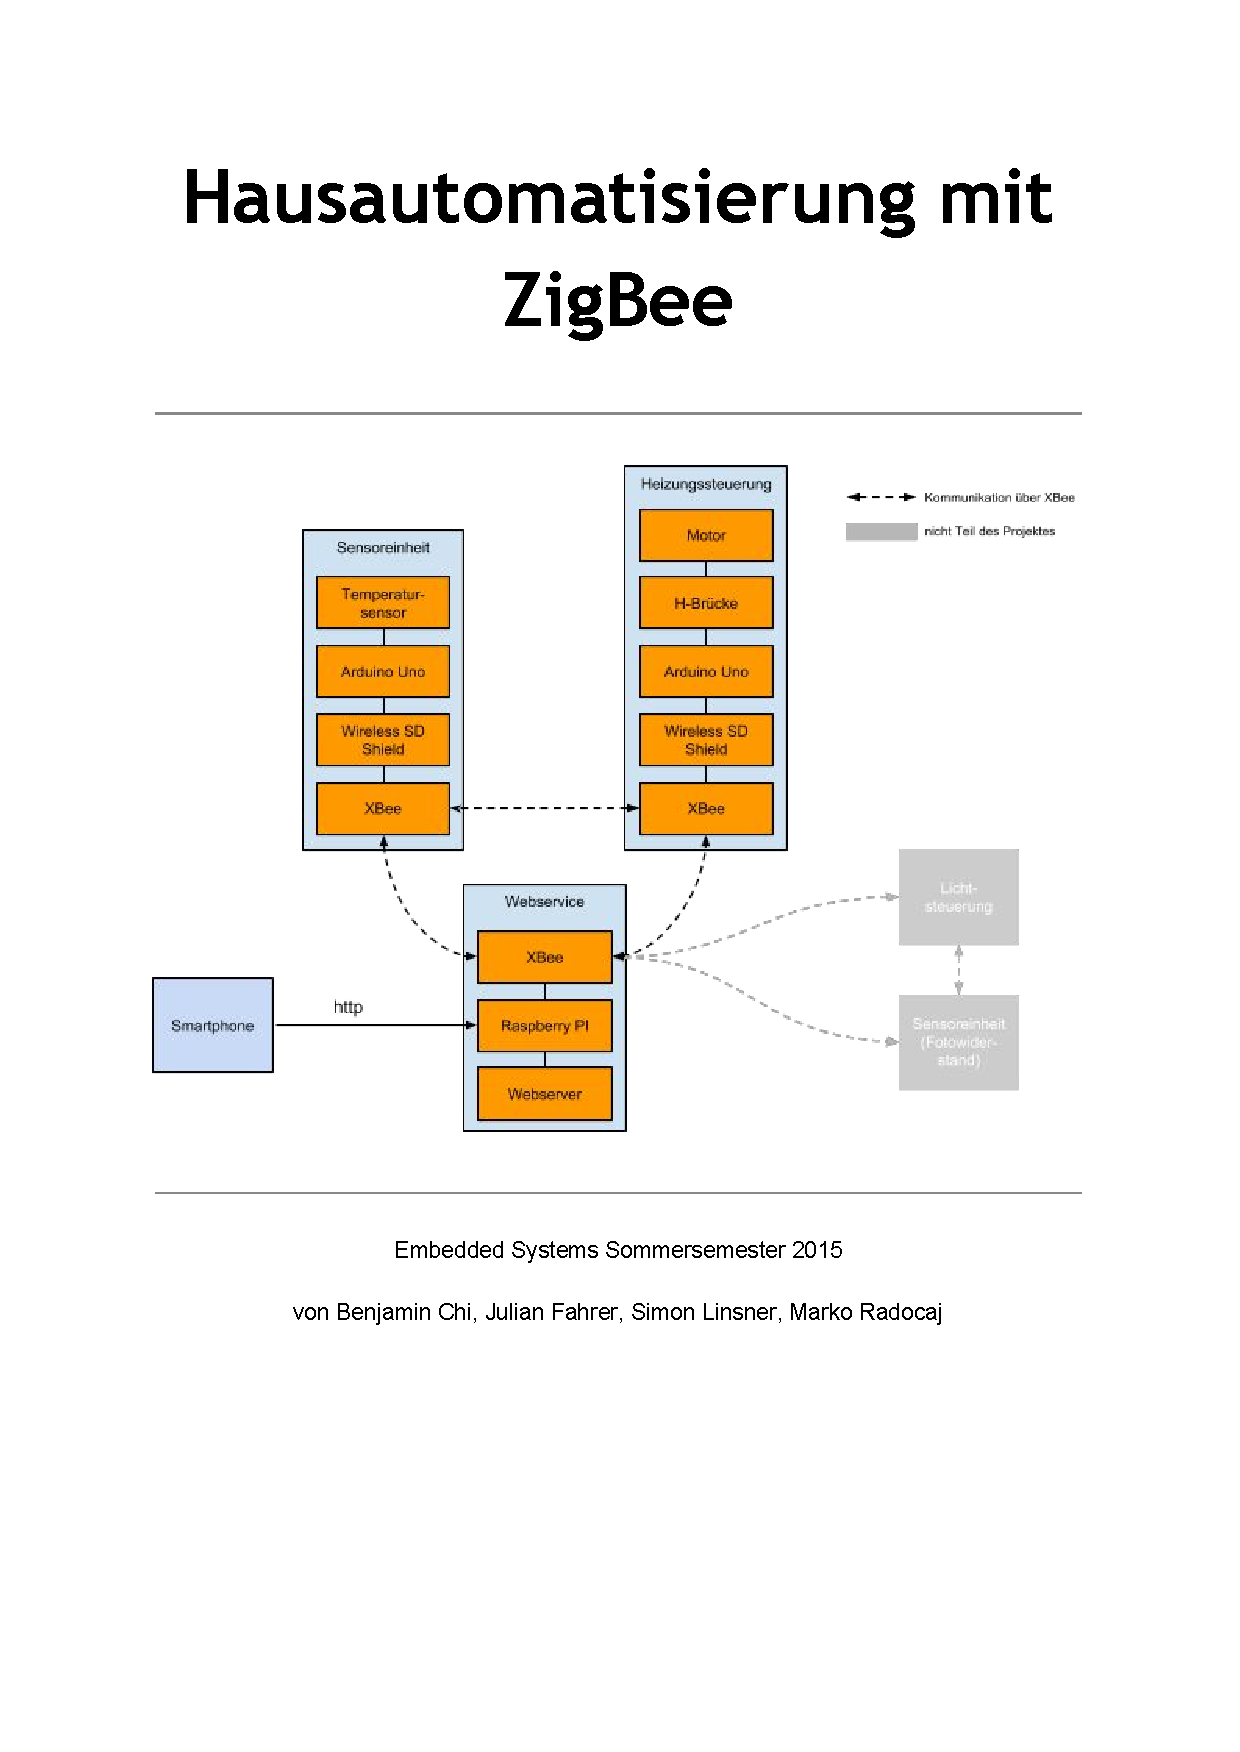
\includepdf[pagecommand={\thispagestyle{headings}},
%  pages=1-23, scale=0.8, frame=true]{Anhang/Dokumentation_SoSe2015.pdf}



\end{document}
